\documentclass[]{scrartcl}

%opening
\usepackage[round]{natbib}
\usepackage{listings}
% \usepackage{minted}
\usepackage{color}
\usepackage{algorithm}
\usepackage{algpseudocode}
\usepackage{amsmath}
\usepackage{amssymb}
\usepackage{dsfont}
\usepackage{pgf}
\usepackage{subcaption}
\usepackage{tikz}
\usepackage{hyperref}
\usepackage{dsfont}
\usetikzlibrary{bayesnet}
\newcommand{\iden}{\ensuremath{\mathbb{I}}}  %identity func
\newcommand{\real}{\ensuremath{\mathbb{R}}} %real numbers
\newcommand{\nat}{\ensuremath{\mathbb{N}}}  %natural numbers
\newcommand{\ints}{\ensuremath{\mathbb{Z}}}
\newcommand{\expt}{\ensuremath{\mathbb{E}}}
\newcommand{\X}{\ensuremath{\mathbb{X}}}
\newcommand{\Z}{\ensuremath{\mathfrak{Z}}}
\newcommand{\y}{\textbf{y}} 
\newcommand{\x}{\textbf{x}} 
\newcommand{\asto}{\overset{a.s.}{\to}}
\renewcommand{\labelitemii}{$\star$}
\newcommand{\om}{\textit{OpenMalaria}}
\DeclareMathOperator*{\argmax}{arg\,\!max}

\title{Notes on Open Malaria}
\author{Bradley Gram-Hansen}

\begin{document}

\maketitle

\begin{abstract}

\end{abstract}

% \input{mognotes/mixofgauss}

\section{What is Open Malria?}
Open malaria is for simulating malaria epidemology and the impacts on that epidemiology of interventions against malaria. 
 It is based on microsimulations of Plasmodium falciparum malaria in humans, originally developed for simulating malaria vaccines.
 These models simulate the dynamics of malaria parasitaemia in the course of an infection, of transmission, of immunity, and of the processes leading to illness and death. The system is set up to simulate malaria in village, or district size human populations

The original models were designed for simulating the impact of interventions acting on humans(for example, chemotherapy, or vaccines). OpenMalaria has subsequently been extended to include simulation of the dynamics of malaria in the mosquito vector, and of interventions that act on mosquitoes. It also offers alternative model structures for many of the components of the human models. The models allow for variations among humans in their exposure to mosquitoes, and in their responses to the parasite.

\section{Facts about Malaria}

\begin{itemize}
\item Endemic in 99 countries, 219 million cases, 660,000 deaths 
\item 90\% in Africa
\item Mortality rates fell by 26\% around the world in the past decade

\section{Simulation Options}

The \om simulator is designed for simulating individual scenarios. 
In order to simulate a study covering variations in several factors, one 
would have to  design a fully \textit{factorial} experiment.

\begin{quote}
	\begin{itemize}
		\item \textbf{\textit{Sweep}} : A sweep is one of more covarying factors, and set of all \textit{arms} of this sweep.
		\item \textbf{\textit{Arm}}: Each sweep must have one or more values for each of its factors. An \textit{arm} 
		is one of these combinations of values - a configuration assigning a value to each factor on the sweep. 
		\item \textbf{\textit{Experiment}}: Largely synonymous with a study, an \textit{experiment} is the complete
		description of all sweeps and arms used, together with the scenarios generated and results produced. Each scenario is generated by choosing
		one arm for each sweep in the experiment. 
		\item \textbf{\textit{Full factorial design}} : A \textit{full factorial experiment} is one where all possible scenarios are generated: all
		combinations of one arm per sweep are used.
		\item \textbf{\textit{Seed}}: Each time a scenario is simulated, the random number generated must be started from some \textit{seed}.
	\end{itemize}
\end{quote}


Since OpenMalaria simulations are stochastic, they use a number of random seeds (say 2-50) 
to provide estimates of the contributions of random variation to the results.

\section{XML files}

Within the open malaria simulator \textit{XML} files should be seen as the program, specifying a model over all parameters. Well kind of, it should actually be treated as a prior to the simulator, providing knowledge regarding how a model is specified in terms of the initial parameters. This then interacts directly with the simulator. 


\section{Key features of the simulator}

\begin{itemize}
\item Seasonality of transmission
\item Access to treatment an inherent part of model
\item Addressing uncertainty: ensemble of 14 model variants

\end{itemize}
\section{How to Use Open Malaria}

\paragraph*{Objectives}
\begin{itemize}
	\item Understand OpenMalaria workflow to design an experiment
	\item Understand the important features of OpenMalaria
	\item Understand, the topic of choice, the model assumptions and how interventions interact 
	\item Understand what information is needed to parameterize OpenMalaria and where to find it
\end{itemize}


\subsection{Seasonality of transmissions}
The Plasmodium falciparum entomological inoculation rate (Pf EIR) is a measure of exposure to infectious mosquitoes. 
When describing transmissions, the simulator is driven by the input value of annual average EIR, the average number of infectious bites a person receives each year.
The seasonality is specifically specified by 12 monthly values for each vector species. Abs values or proportion for each month.

In epidemiology, a \textbf{disease vector} is any agent that carries and transmits an infectious pathogen into another living organism; most agents regarded as vectors are organisms, such as intermediate parasites or microbes, but it could be an inanimate medium of infection such as dust particles.

\section{How does Malaria spread?}
\begin{itemize}
\item Deterministic model of malaria transmission based on the mosquito feeding cycle
\item Linked to models of interventions
\item Driven by EIR
\item For input EIR values, you may need to work backwards to determine pre-experiment level
\end{itemize}


\begin{figure}
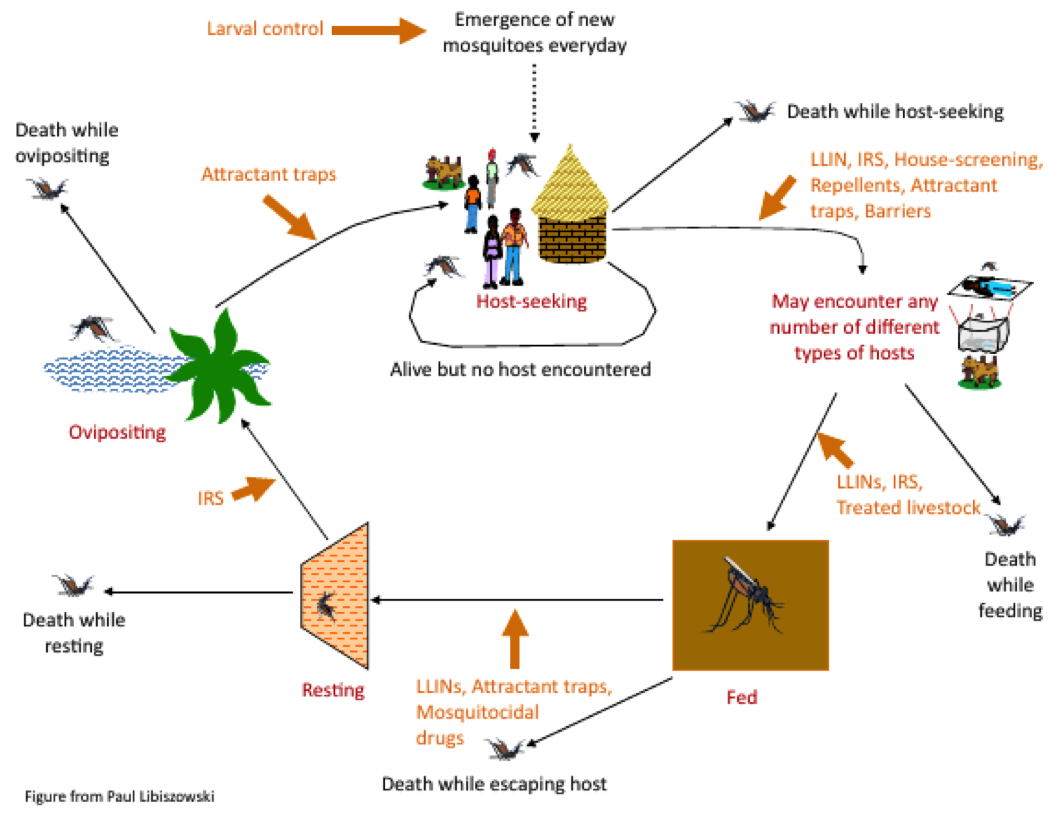
\includegraphics[width=\textwidth]{images/malariacycle.png}
\caption{The mosquito feeding cycle. Malaria is spread through this cycle.}
\end{figure}

\section{Modelling different treatments}

Stochastic simulation models of malaria based on the simulation of infections in humans. Tracks health status of individuals at discrete time points

\begin{figure}
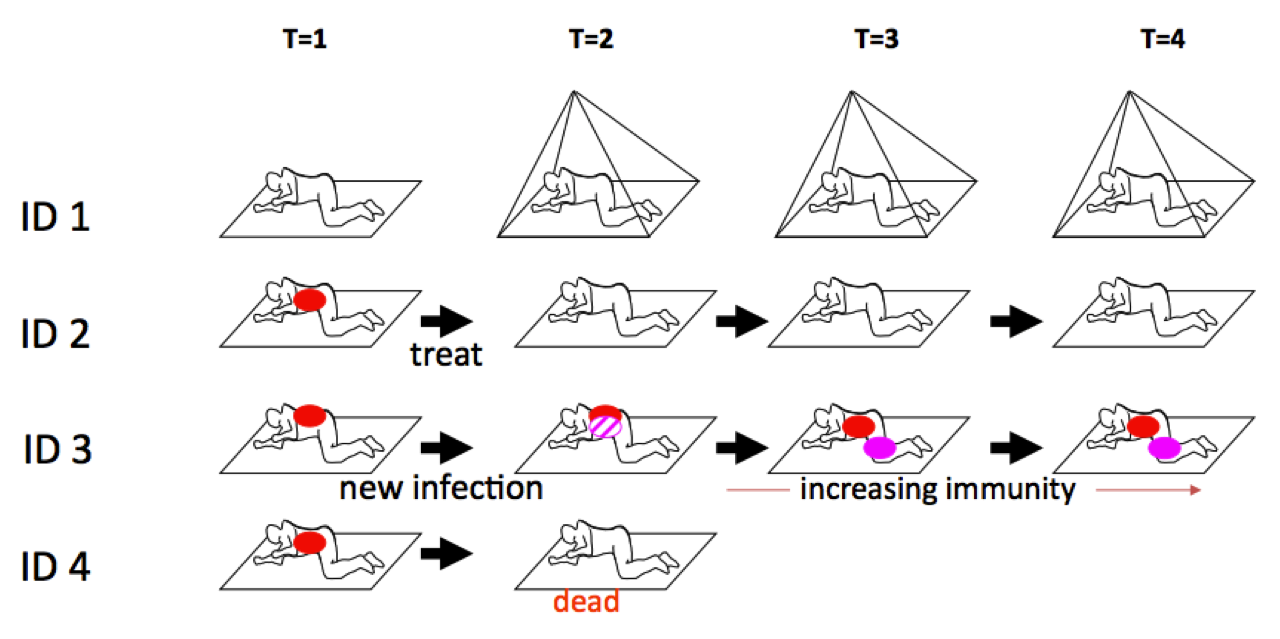
\includegraphics[width=\textwidth]{images/malariatreatment.png}
\end{figure}

\begin{figure}
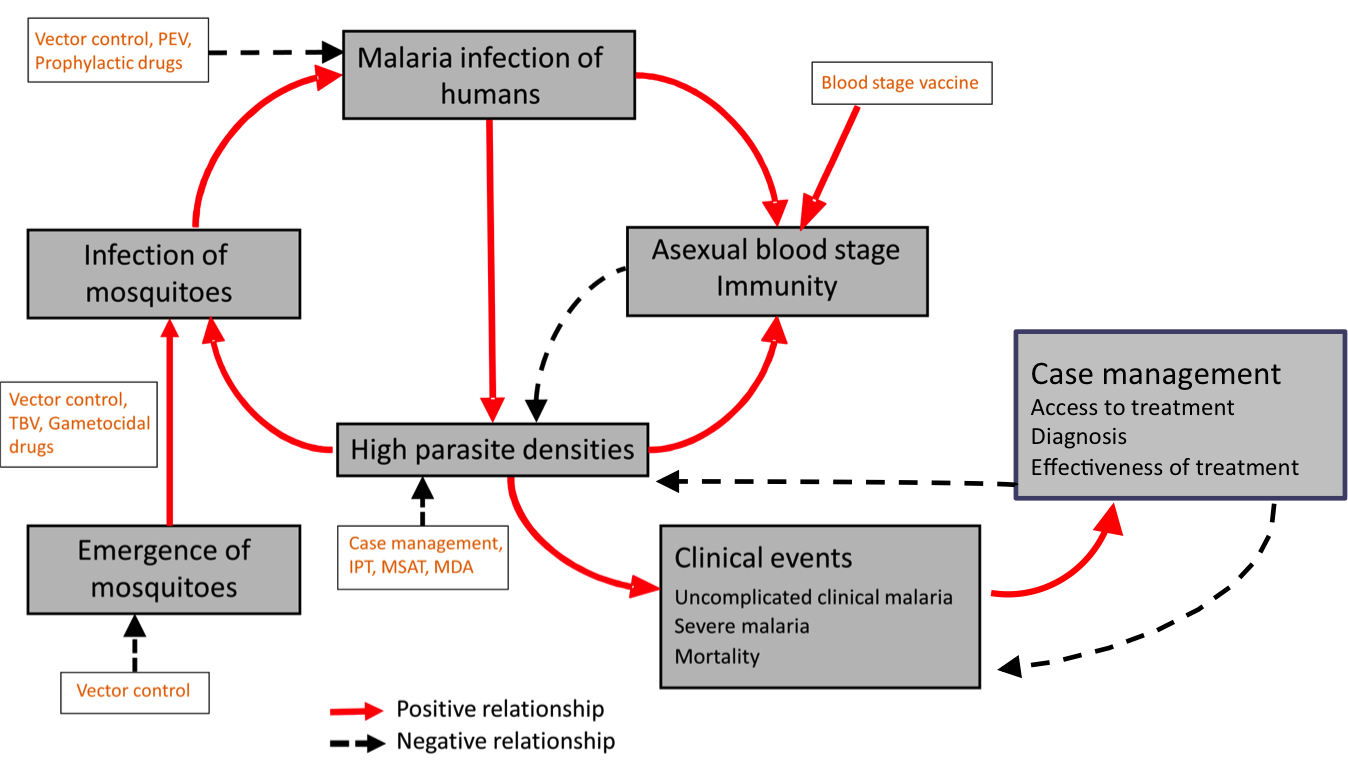
\includegraphics[width=\textwidth]{images/accesstotreatment.png}
\end{figure}
\section{Scenario transmission}


OpenMalaria simulations of malaria transmissions require a specification of:
\begin{itemize}
	\item The level and seasonality of exposure (measured by the Entomological Inoculation Rate, EIR) to malaria at the start of the simulation
	\item The model for transmission from mosquitoes to humans and the dynamics of malaria parasite cycle within humans.
	\item The model for malaria transmission from humans to 
	\item The entomological model. There are two different variants of the entomological model:
	\begin{itemize}
    \item The "Non-vector" variant does not consider mosquito dynamics and hence uses fixed or periodically (seasonally) varying vectorial capacity. It is appropriate for modeling situations with only interventions such as chemotherapy or vaccines that only act on humans.
	\item The "Vector" variant comprises discrete-time population models that simulate how many mosquitoes belong in each of several categories at each time. The models assume that the infectious (sporozoite positive) mosquitoes act to distribute infections at random to the human population (with human exposure proportionate to availability). Entomological interventions modify the vectorial capacity and require the "vector" transmission model variant. The simulations that include non-periodic changes in the vectorial capacity use a seasonally forced version of the difference equation model for vector dynamics.
\end{itemize}
\end{itemize}

\section{Tom stuff}

\paragraph*{Tom notes}

\begin{itemize}
	\item Always write down an abstract and introduction when you are starting a new project. 
	\item Write down ideas as formally as possible. 
	\item Things that happen first - the less applied part: 
	\begin{itemize}
		\item As you mathematically formulate in code, you write down the mathematics that describes that and the problem formulation. 
         \item Try and write down a joint of the model. That way you can determine if the problem is doable. Must deal with these things first. 
\end{itemize}
\end{itemize}

Things to look into:

\begin{itemize}
\item Are there Multi-modes?
\item Is the problem high-dimensional?
\item What is the dimensionality of problems?
\end{itemize}


\subsection{Approximate Bayesian Computation}

When dealing with a constrained set of distributions we can perform exact Bayesian inference, that is we can use statistically correct inference algorithms to find the true posterior $p(x | D) = \frac{p(D|x)p(x)}{p(D)}$, not just heuristic results. If we choose the a conjugate-pair of prior $p(x)$ and likelihood function $p(x|D)$ then we can also analytically exactly calculate the true posterior. However, in general most real world problems, i.e. physically simulations, cannot necessarily be constrained to this family of problems, as the likelihood is typically intractable, or computationally expensive to compute. This occurs because the \textit{forward simulator} emulates the likelihood function
due to the ingrained stochasticity with the model, which makes it impossible to write down a likelihood function. Nonetheless, we can still apply a series of approximation techniques, such as variational inference that enable one to approximate the true posterior. Although such algorithms typically have no guarantees, they are typically lower bounded.   


\subsection{Applied Interpretable Inference}


\section{Gunes Notes}
\begin{itemize}
	\item ABC - talk about this in the context to MCMMC
	\item The forward simulator represents some likelihood function that can be tractable or intractable. 
	\item Within forward simulators the randomness comes from rejection sampling statements , but conditioning within the simulators is hard
this is why we need to use the prob prog system . 
\end{itemize}

\end{document}


